\documentclass[fontsize=12pt]{article}
\usepackage{amsmath}
\usepackage[a4paper, total={5in, 9in}]{geometry}
\usepackage{graphicx} 
\usepackage{cite}
\usepackage[hidelinks]{hyperref}
\usepackage{adjustbox}
\usepackage[dvipsnames]{xcolor}
\usepackage{marginnote}
\usepackage{booktabs}
\usepackage{gensymb}
\let\marginpar\marginnote
\usepackage{multicol}
\usepackage{float}
\usepackage{acro}
\definecolor{deepnavy}{RGB}{59, 40, 150}
\definecolor{mutedsage}{RGB}{25, 114, 120}
\definecolor{warmterracotta}{RGB}{193, 41, 46}

\let\oldphi\phi
\renewcommand{\phi}{\varphi}

\newenvironment{Figure}
  {\par\medskip\noindent\minipage{\linewidth}}
  {\endminipage\par\medskip}

\hypersetup{
    colorlinks=true,
    linkcolor=deepnavy,
    citecolor=mutedsage,
    urlcolor=warmterracotta,
}
 
\addtolength{\oddsidemargin}{-0.4in}
\addtolength{\evensidemargin}{-0.4in}
\addtolength{\textwidth}{0.8in}
\addtolength{\topmargin}{-.5in}
\addtolength{\textheight}{1.0in}

\DeclareAcronym{llm}{
    short = LLM,
    long = Large Language Model,
    short-indefinite = an,
    long-indefinite = a,
}

\DeclareAcronym{bert}{
    short=BERT,
    long=Bidirectional Encoder Representations from Transformers
}

\setlength{\parindent}{0pt}

\title{ Embeddings and Language Production}
\author{Week 7, Spotted in the Wild}
\date{Tom Cassar}

\begin{document}

%Alongside your submission, you should provide a brief explanation of where/how you encountered it and how it's related to the topic of the module.  There's no fixed length for this, but if you need more than 200ish words to explain the connection, consider whether it's really as relevant as it should be. 

\maketitle

While browsing through YouTube before falling asleep last night, I came across a
video from a popular Maths YouTuber 
\href{https://www.youtube.com/@3blue1brown}{3blue1brown}. The thumbnail (Figure
\ref{fig:thumbnail}) showed a
lot of vectors, and the title was ``\textit{How might LLMs store facts}''. The
video was part of a wider series on the maths underpinning large language
models, of which I had seen an episode or two before. \newline 

\begin{figure}[H]
    \centering
    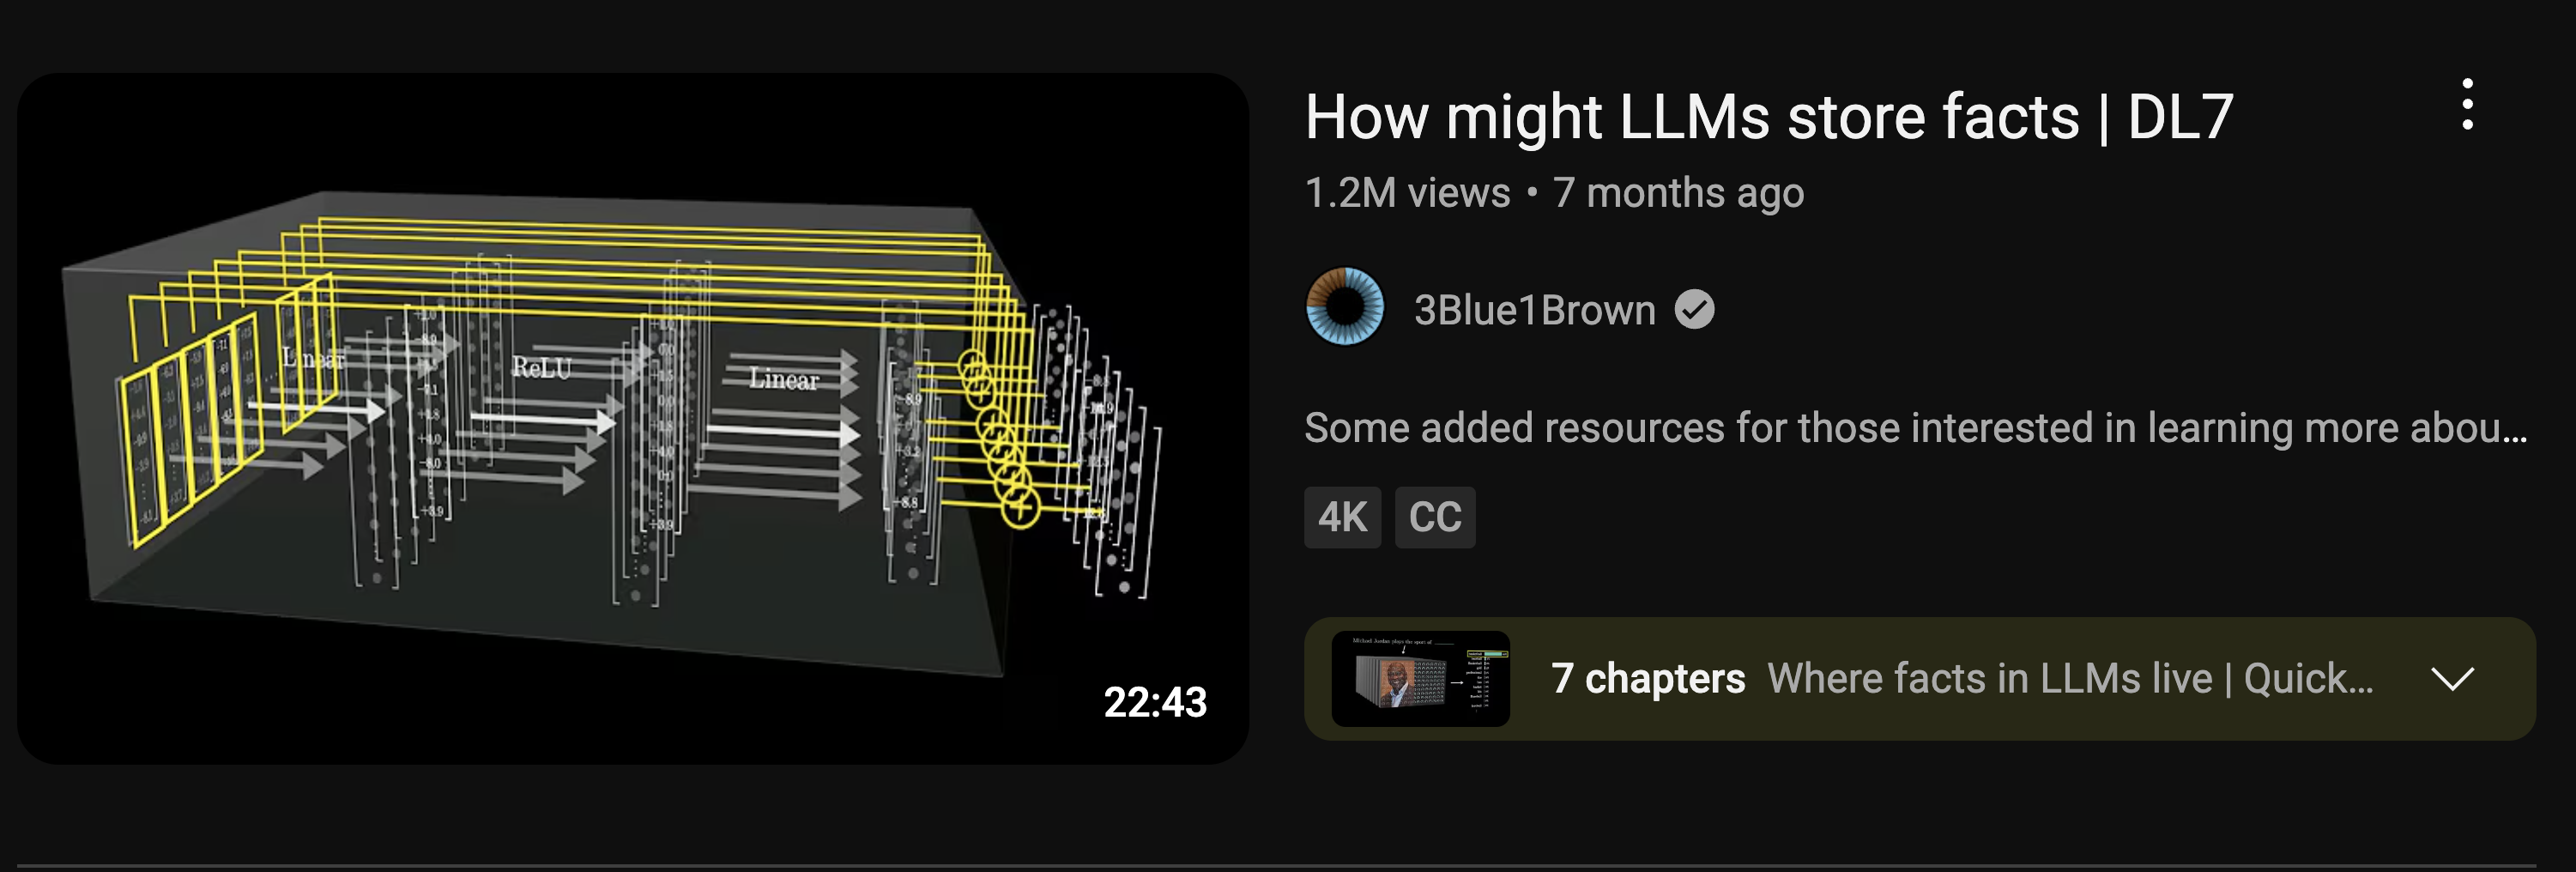
\includegraphics[width=0.8 \linewidth]{./img/thumbnail.png} 
    \caption{The thumbnail of 3blue1brown's video that I saw yesterday evening
    before bed \cite{3Blue1Brown_2024}.}
    \label{fig:thumbnail}
\end{figure}

The video discussed how \acp{llm} represents information internally. The toy
problem presented explores how \iac{llm} represents and reasons about the
concept of Lebron James. It turns out that \iac{llm} doesn't store words
but \textbf{embeddings}: mathematical encodings of \textbf{meaning}. In some
implementations such as \texttt{word2vec}, these embeddings can be meaningfully
manipulated: $\text{king} - \text{man} + \text{woman} \approx \text{queen}$
\cite{tensorflow_word_embeddings}. \newline

This reminded me of the content in Week 7: specifically, how language errors can
be used to provide insight into how we encode language in our brains. The key
similarity is that neither we nor \acp{llm} seem to encode meaning in terms of
actual words, but some other more abstract means. \newline

Some language errors which were given as evidence for this abstract
representation were \textit{spoonerisms}, \textit{tongue twisters}, and
\textit{tip of the tongue} errors. Another was \textit{agreement errors}: since
\acp{llm} also use an abstract representation for language, I wondered if they
too were susceptible to agreement errors. It seems that to an extent, they are -
especially \acp{llm} based on \ac{bert} \cite{bazhukov-etal-2024-models}.

\bibliographystyle{vancouver}
\bibliography{embeddings-and-language-errs}

\end{document}
